\section{Remote Produre Calls}
Die RPCs sind mit einem Trait 'Calls' zur Bestimmung der Signaturen aller remote rufbaren Funktionen der Container deklariert.
Zur Kommunikation nutzen wir TCP Sockets über die wie folgendens Nachrichten zum Funktionsaufruf als bytes codiert gesendet werden:

\begin{figure}[H]
    \centering
    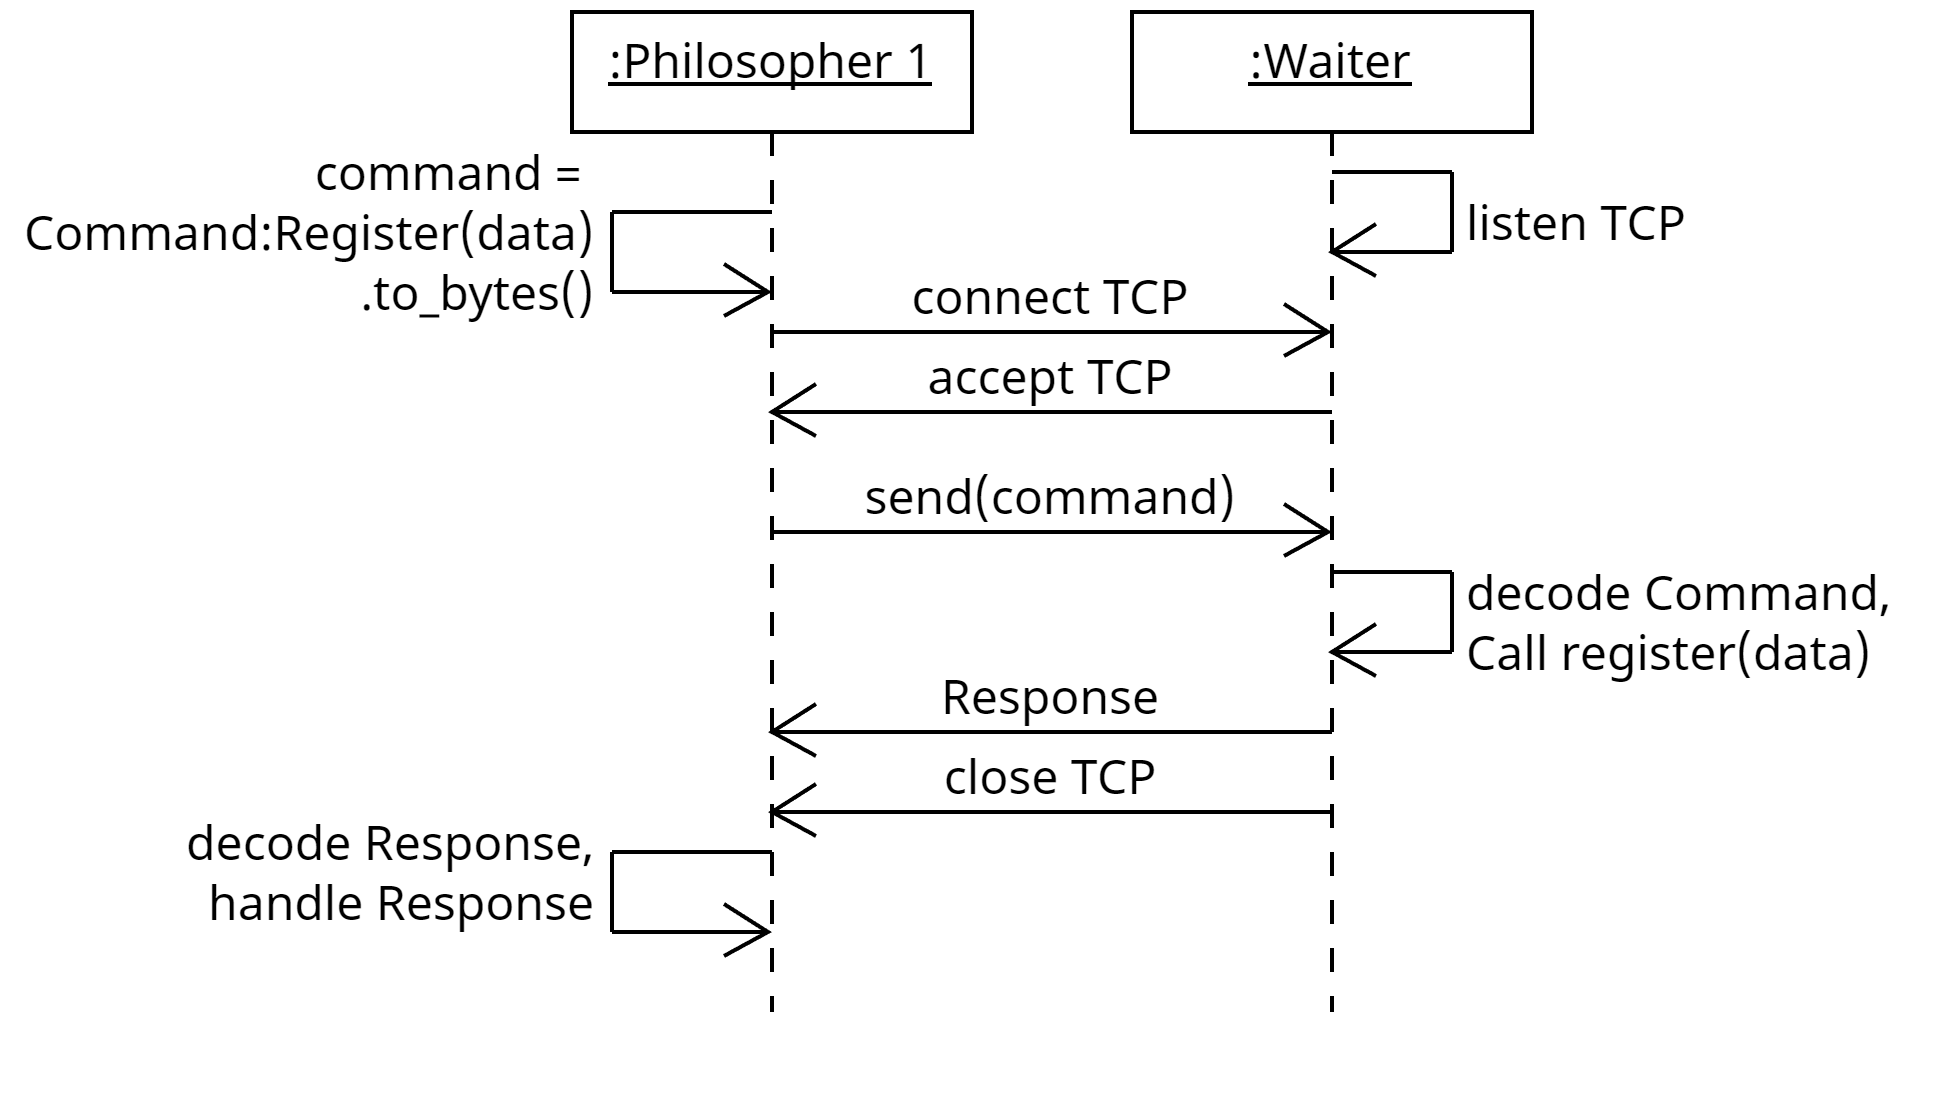
\includegraphics[width=0.7\textwidth]{images/rpc.png}
    \caption{RPC Ablauf}
    \label{fig:setup}
\end{figure}

\begin{itemize}
    \item \textbf{Commands} ist ein enum das alle möglichen Funktionsaufrufe an Nodes umfasst und beim Senden eines RPCs in bytes codiert und gesendet wird und anschließend vom Empfänger ins enum decodiert und als Funktionsaufruf ausgeführt wird.
    \item Das Antwortformat auf einen RPC ist ein enum \textbf{Response}: { Success, Failure(String), Return(Vec<u8>)}, das je nach Ausgang des Aufrufs Daten zurückliefern kann.
\end{itemize}
